\subsection{Massimi e minimi}

\subsubsection{Massimi e minimi locali}

Vediamo ora alcuni concetti che ci serviranno poi per i problemi di ottimizzazione vincolata.

\defn{Massimo e minimo locale}{

    Sia \(f: D \subseteq \Rn \to \R \), dove \(D\) è il dominio, ovvero l'unione dei punti dell'insieme aperto con quelli della frontiera.

    Si dice che \(\ux_0 \in D\) è un punto di \textbf{minimo locale} (o \textbf{relativo}), se esiste un intorno sferico \(B(\ux_0, \sigma) \), con \(\sigma > 0\), tale che:

    \[
        f(\ux_0) \le f(\ux) \quad \forall \ux \in D \cap B(\ux_0, \sigma)
    \]

    La definizione è analoga per il punto di massimo locale.
}

\defn{Massimo/Minimo stretto}{
    Il punto di minimo o massimo locale si dice \textbf{stretto} se la disuguaglianza è strettamente minore o strettamente maggiore.
}

\defn{Massimo/Minimo globale}{
    Un punto di massimo/minimo, si dice \textbf{globale} (o \textbf{assoluto}) se la disuguaglianza vale per tutto il dominio, ovvero \(\forall \ux \in D\) e non solo per l'intorno sferico di centro \(\ux_0\) e di raggio \(\sigma \).
}

Da Analisi 1 sappiamo che i punti di minimo e massimo vanno ricercati fra i punti stazionari, ovvero nei punti critici, di funzioni differenziabili, in cui il gradiente si annulla.

Se \(\ux_0\) è punto di minimo (massimo) locale interno a \(D\) (quindi \(\ux_0 \in D\)) allora vale l'estensione in più variabili del Teorema di Fermat.

\filbreak{}
\teorema{Teorema di Fermat per funzioni in più variabili}{
    Sia \(f:D \subset \Rn \to \R \);

    Sia \(\ux_0 \in D\) punto di estremo locale per \(f\);

    Se \(f\) è differenziabile in \(\ux_0\), allora, \(\nabla f(\ux_0) = 0\)
}
\begin{proof}
    Supponiamo \(\ux_0\) punto di massimo relativo. Allora \(\ux_0\) è punto di massimo relativo anche per la restrizione di \(f\) lungo una qualsiasi retta passante per \(\ux_0\).

    Consideriamo il versore \(\underline{v} \in \Rn \) come il vettore di norma 1 che ci indica la direzione di tale retta passante per \(\ux_0\). I punti su tale retta sono quindi della forma \(\ux_0 + t\underline{v}\) per \(t \in \R \).

    Definiamo la funzione \(F: \R \to \Rn \) che associa \(t \mapsto f(\ux_0 + t\underline{v})\). Questa funzione \(F(t)\), è una funzione in \textbf{una variabile} e diciamo che sia almeno definita in un intorno di \(t=0\).

    Ora, siccome \(\ux_0\) è punto di massimo per \(f\), allora in \(t=0\) abbiamo un punto di massimo per \(F\). Quindi per il teorema di Fermat in una variabile: \(F'(0) = 0\).

    Se quindi espandiamo \(F'(t)\) con la regola della catena, per qualsiasi direzione \(\underline{v}\) otteniamo:

    \[
        F'(t) = \prods{\nabla f(\ux + t\underline{v})}{\underline{v}}
    \]
    \[
        F'(0) = 0 = \prods{\nabla f(\ux_0)}{\underline{v}}
    \]

    E siccome \(\norm{\underline{v}} = 1\), allora \(\underline{v} \neq \uzero \), allora necessariamente \(\nabla f(\ux_0) = 0\).

\end{proof}

\filbreak{}
\defn{Punti stazionari (o critici)}{
    I punti \(\ux_0 \in A\) tali che \(\nabla f(\ux_0) = 0\) si dicono \textbf{punti stazionari} (o critici) di \(f\) in \(A\).
}

\defn{Sella (o colle)}{
    Essere un punto stazionario, è condizione necessaria ma non sufficiente per essere un punto di estremo.

    In funzioni a una variabile, un punto stazionario che non era però un punto di estremo lo chiamavamo flesso;

    In funzioni a più variabili, un punto stazionario che non è però un estremo relativo viene chiamato \textbf{sella} (o colle).
}

Un esempio classico di punto di sella, è il punto \((0,0,0)\) nella funzione \(z=x^2-y^2\):
\begin{center}
    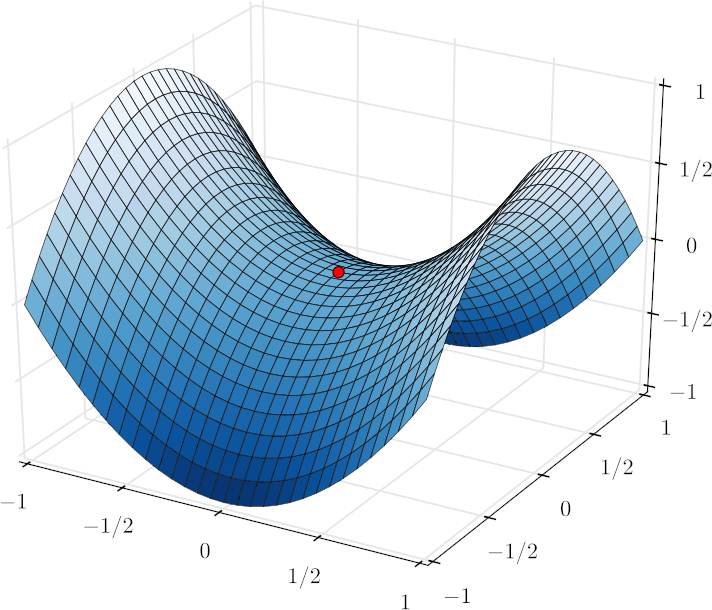
\includegraphics[width=0.5\textwidth]{punto-di-sella.png}
\end{center}

\filbreak{}
\subsubsection*{Esercizio 1}

Cercare i punti critici della seguente funzione:

\[
    f(x,y) = 2x^{2} - 2xy +y^{2}
\]

Cerco i punti dove \(\nabla f(x,y) = 0\):
\begin{align*}
     & f_x = 4x -2y  \\
     & f_y = -2x +2y
\end{align*}

\[
    \begin{cases}
        4x -2y = 0 \\
        -2x +2y = 0
    \end{cases}
    \implies
    \begin{cases}
        x = 0 \\
        y = 0
    \end{cases}
\]

Quindi, \(\ux_0 = (0,0)\), è un punto critico \(\implies \nabla f(\ux_0)=0\)

Inoltre, possiamo osservare che:

\[
    f(x,y) = x^{2} + {(x-y)}^{2}
\]

è una somma di due quadrati, quindi:

\[
    f(x,y) > f(0,0) ~\forall (x,y) \neq (0,0)
\]

Quindi si ha che \(\ux_0 = (0,0)\) è un punto di \textbf{minimo globale stretto}.

\subsubsection*{Esercizio 2}

Cercare i punti critici della seguente funzione:

\[
    f(x,y) = x^{2}-y^{2}
\]

\[
    \nabla f(x,y) = (2x, -2y)
\]

anche qui \((0,0)\) è l'unico punto critico. Questo punto è però un punto di sella, infatti, se consideriamo gli incrementi lungo gli assi:
\begin{itemize}
    \item Lungo l'asse x: \(f(x,0) = x^{2} \ge 0 ~\forall x\)
    \item Lungo l'asse y: \(f(0,y) = -y^{2} \le 0 ~\forall y\)
\end{itemize}
abbiamo un cambiamento di segno dentro l'intorno sferico \(B(\uzero, r)\) e quindi \(\ux_0\) non è ne un massimo ne un minimo.

Come vedremo tra poco, questa conclusione è possibile trarla anche facendo un'analisi dell'incremento subito dalla funzione:
\[
    \Delta f(x,y) = f(x,y) - f(0,0) = x^{2}-y^{2}-0 \quad\forall (x,y) \in B(\uzero,r),\ r>0
\]
da cui si nota che a seconda del valore di \((x,y)\) si ha un cambiamento di segno, e quindi abbiamo un punto di sella.

\pagebreak
\subsubsection{Forma quadratica}

Prima di passare al prossimo argomento è necessario introdurre la notazione di ``Forma quadratica''.

Per un vettore \(\ux \in \Rn \), una forma quadratica è un polinomio omogeneo di secondo grado nelle variabili \((x_1,\ldots,x_n)\):

\[
    q(\ux ) = q(x_1,\ldots,x_n) = \sum^{n}_{i,j=1} a_{ij} x_i x_j
\]

Quindi, se consideriamo la matrice dei coefficienti \(A = (a_{ij})\), possiamo scrivere ogni forma quadratica come:

\[
    q(\ux ) = \prods{A\ux}{\ux}
\]

Da qui, notiamo che tutti gli \({x_i}^{2}\) hanno come coefficiente \(a_{ii}\), ovvero i coefficienti che stanno sulla diagonale di \(A\).

\subsubsection*{Esempio}

Sia \(n=2\); \(\ux =(x_1,x_2)\); \(A\) simmetrica.

Sappiamo in generale che:

\[
    q(x_1,x_2) = a_{11} {x_1}^{2} + 2a_{12} x_1 x_2 + a_{22}{x_2}^{2}
\]

per una matrice \(2\times 2\):

\[
    A= \begin{pmatrix}
        1 & 5 \\
        5 & 4
    \end{pmatrix} \iff
    q(x_1,x_2) = {x_1}^{2}+4 {x_2}^{2}+ 10 x_1 x_2
\]

per una matrice \(3\times 3\):

\[
    A = \begin{pmatrix}
        2  & -2 & 5 \\
        -2 & 3  & 0 \\
        5  & 0  & 4
    \end{pmatrix} \iff
    q(\ux ) = 2 {x_1}^{2}+3 {x_2}^{2}+ 4 {x_3}^{2} - 4 x_1 x_2 + 10 x_1 x_3
\]

\subsubsection*{Definizione sul segno}

Sia \(n=2\); per una data matrice dei coefficienti \(A = (a_{ij})\); la forma quadratica \(q: \ux \mapsto \prods{A\ux}{\ux}\)
\begin{itemize}
    \item si dice \textbf{definita positiva} se \(\forall \ux \neq 0\) si ha \(q(\ux ) >0\)
    \item si dice \textbf{definita negativa} se \(\forall \ux \neq 0\) si ha \(q(\ux ) <0\)
    \item si dice \textbf{indefinita} se \(\exists x_1, x_2 \in \R^{2} \giventhat q(x_1) < 0 < q(x_2)\), ovvero cambia il segno
\end{itemize}

\pagebreak
\subsubsection{Classificazione dei punti critici {-} Matrice Hessiana}

\proposizione{Test dell'hessiana}{

Sia \(f: D \subseteq \R^{2} \to \R \), \(D\) aperto con \(f \in C^{2}(D)\)

Sia \((x_0,y_0) \in D\) un punto critico per \(f\), ovvero tale che \(\nabla f(x_0,y_0) = 0\)

Sia il determinante della matrice Hessiana \(\neq 0\), ovvero:
\[
    \det (Hf(x_0,y_0)) =
    \left| \begin{matrix}
        f_{xx}(x_0,y_0) & f_{xy}(x_0,y_0) \\
        f_{xy}(x_0,y_0) & f_{yy}(x_0,y_0)
    \end{matrix} \right| =
    f_{xx}(x_0,y_0) f_{yy}(x_0,y_0) - {f_{xy}}^{2}(x_0,y_0)
    \neq 0
\]

Allora:

\begin{itemize}
    \item Se \(\det(Hf(x_0,y_0))>0\) e \(f_{xx}(x_0,y_0)>0 \implies (x_0,y_0)\) è punto di minimo locale
    \item Se \(\det(Hf(x_0,y_0))>0\) e \(f_{xx}(x_0,y_0)<0 \implies (x_0,y_0)\) è punto di massimo locale
    \item Se \(\det(Hf(x_0,y_0))<0 \implies (x_0,y_0)\) è un punto di sella
\end{itemize}
}

Osservazione: se \(\det(Hf(x_0,y_0)) =0\) il test dell'hessiana \textbf{non} ci fornisce informazioni. Devo quindi fare un'analisi diretta dell'incremento subito dalla funzione, ovvero:
\[
    \Delta f(x,y) = f(x,y)-f(x_0,y_0) \qquad \forall (x,y) \in D \cap B(x_0,y_0)
\]

\begin{proof}
    Questa dimostrazione è basata sull'approssimazione al secondo ordine della nostra funzione in \(\ux = (x_0, y_0)\), attraverso la formula di Taylor al II ordine col resto di Peano:

    \[
        f(\ux + \uh ) = f(\ux ) + \prods{ \nabla f(\ux )}{\uh} + \frac{1}{2} \prods{ Hf(\ux ) \cdot \uh}{\uh} + o(\norm{\uh}^{2})
    \]

    Se consideriamo l'approssimazione nel punto \(\ux = (x_0,y_0)\), ricordando che per ipotesi \(\ux \) è punto critico e quindi \(f_x(\ux)=0=f_y(\ux)\), abbiamo dunque che:
    \begin{align*}
        f(\ux + \uh)          & = f(\ux) + 0 + \frac{1}{2} \prods{ Hf(\ux ) \cdot \uh}{\uh} + o({\norm{\uh}}^2) \\
        f(\ux + \uh) - f(\ux) & = \frac{1}{2} \prods{ Hf(\ux ) \cdot \uh}{\uh} + o({\norm{\uh}}^2)              \\[2mm]
        f(x,y) - f(x_0,y_0)   & = \frac{1}{2} \prods{ Hf(\ux ) \cdot \uh}{\uh} + o({\norm{\uh}}^2)
    \end{align*}
    Osserviamo che, \(\frac{1}{2} \prods{ Hf(\ux ) \cdot \uh}{\uh}\), è un polinomio di II grado in \(\uh=(h,k)\), i cui coefficienti sono le derivate seconde di \(f\), che esistono per ipotesi.

    In generale, questo polinomio è sempre una forma quadratica, \(q(\uh)\) con {\(\uh \in \Rn \)}, quindi un polinomio omogeneo di secondo grado nelle variabili \((h_1,\ldots,h_n)\).

    Ricordando che \(q(\uh) = \prods{A\uh}{\uh}\), nel nostro caso la matrice associata \(A\) è proprio la matrice Hessiana, che è pure simmetrica per il teorema di Schwarz (ipotesi iniziali: \(f \in C^{2}(D)\)).

    Studiare il segno di \(\Delta f(x,y)\), ovvero il segno della funzione nell'intorno del punto critico, è quindi uguale a studiare il segno di questa quadratica hessiana.

    Per la regola di Cartesio, per studiare il segno della quadratica hessiana possiamo usare il segno degli autovalori. Vediamo quindi cosa succede:

    \begin{itemize}
        \item \(\det(Hf(\ux))>0,\ f_{xx}(\ux)>0 \implies \) forma quadratica è definita positiva \(\implies \ux \) è minimo
        \item \(\det(Hf(\ux))>0,\ f_{xx}(\ux)<0 \implies \) forma quadratica è definita negativa \(\implies \ux \) è massimo
        \item \(\det(Hf(\ux))<0 \implies \) forma quadratica è indefinita \(\implies \ux \) è punto di sella
    \end{itemize}

\end{proof}

\subsubsection*{Esercizio 1}

Classificare i punti critici delle seguenti funzioni:

\[
    f(x,y) = 2x^{3}-6xy + 3y^{2}
\]

\[
    \nabla f(x,y)=0 \implies \begin{cases}
        6x^{2}-6y=0 \\
        -6x + 6y =0
    \end{cases}
    \implies
    (x,y) \in \{(0,0), (1,1)\}
\]

Test dell'hessiana:

\[
    f_{xx}(x,y) = 12x
\]
\[
    f_{xy}(x,y) = -6
\]
\[
    f_{yy}(x,y) = 6
\]

quindi:

\[
    H f(x,y) = \begin{bmatrix}
        12x & -6 \\
        -6  & 6
    \end{bmatrix}
\]

gli sostituiamo i punti trovati prima:

\[
    Hf(0,0) = \begin{bmatrix}
        0  & -6 \\
        -6 & 6
    \end{bmatrix}
\]

quindi:

\[
    \det (Hf(0,0)) = -36 <0 \implies (0,0) \text{ punto di sella}
\]

\[
    Hf(1,1) = \begin{bmatrix}
        12 & -6 \\
        -6 & 6
    \end{bmatrix}
\]

quindi:

\[
    \det (Hf(1,1)) = 36 >0 \text{ e } f_{xx}(1,1) = 12 > 0 \implies (0,0) \text{ minimo locale}
\]

\subsubsection*{Esercizio 2}

\[
    f(x,y) = x^{3} + {(x-y)}^{2}
\]

\[
    \nabla f(x,y)=0
    \implies
    \begin{cases}
        3x^{2}+2(x-y) = 0 \\
        -2(x-y) = 0
    \end{cases}
    \implies
    \begin{cases}
        3x^{2}= 0 \\
        x-y= 0
    \end{cases}
    \implies
    (x,y) \in \{(0,0)\}
\]

\[
    f_{xx}(x,y) = 6x+2
\]
\[
    f_{xy}(x,y) = -2
\]
\[
    f_{yy}(x,y) = 2
\]

\[
    H f(x,y) = \begin{bmatrix}
        6x+2 & -2 \\
        -2   & 2
    \end{bmatrix}
\]

\[
    \det(H f(x,y)) = 2(6x+2) - 4
\]
\[
    \det(H f(0,0)) = 4-4 = 0
\]

Quindi non posso applicare il test dell'hessiana.

Allora considero l'incremento in un intorno sferico dell'origine:

\[
    \Delta f(x,y) = f(x,y) - f(0,0) = x^{3}+{(x-y)}^{2} -0 = x^{3}+{(x-y)}^{2}
\]

e dunque, si può escludere che in \((0,0)\) ci sia minimo o massimo relativo perché il segno cambia.

Infatti, questo si vede facilmente ad esempio restringendo la funzione lungo la curva \(y=x\):

\[
    \Delta f(x,x) = x^{3}
\]

questa cambia segno dipendentemente dal valore di \(x\).

Quindi possiamo concludere che \((0,0)\) è un punto di sella.

\pagebreak
\subsubsection{Massimi e minimi su domini limitati e chiusi di \texorpdfstring{\(\R^{2}\)}{R2}}

Nel caso di funzioni su domini limitati e chiusi vale il seguente teorema:

\teorema{Weierstrass}{
    Sia \(f: K \subseteq \R^2 \to \R \) continua; con \(K\) \textbf{limitato e chiuso}.

    Allora \(f\) è \textbf{limitata} e ha minimo e massimo su \(K\), ovvero:

    \[
        \exists (x_0,y_0),(x_1,y_1) \in K \giventhat f(x_0,y_0) \le f(x,y) \le f(x_1, y_1) ~\forall (x,y) \in K
    \]

    ovvero, esiste:
    \begin{itemize}
        \item \(f(x_0, y_0)\) valore minimo assoluto di \(f\) su \(K\)
        \item \(f(x_1, y_1)\) valore massimo assoluto di \(f\) su \(K\)
    \end{itemize}
}
